\textbf{{1.迭代查询}}

当根域名服务器收到本地域名服务器的迭代查询请求报文时,要么给出所要查询的IP地址,要么告诉本地域名服务器``下一步应当向哪一个域名服务器进行查询'',然后让本地域名服务器进行后续的查询,如下图所示。

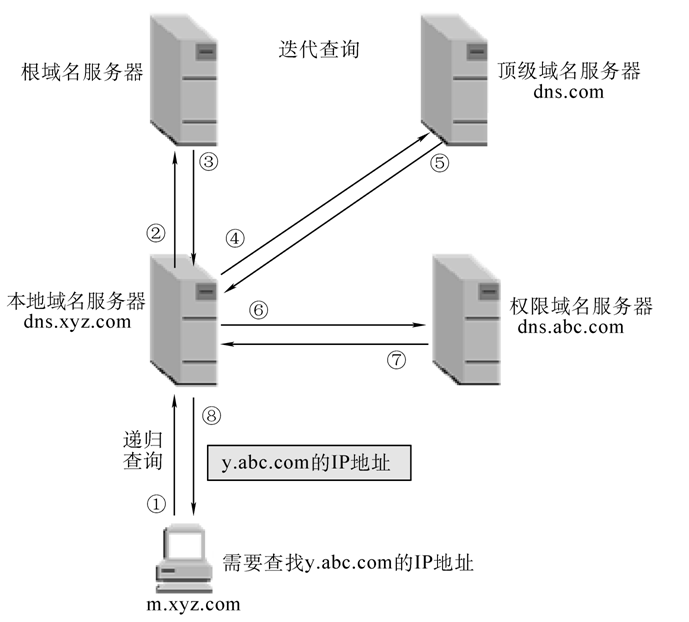
\includegraphics[width=6in]{png-jpeg-pics/E26E2735B3A59AA406F10A089E6A8C0E.png}

{\textbf{注意:}}\textbf{因为主机向本地域名服务器的查询都是采用递归查询,所以迭代查询又称为递归与迭代相结合的查询方式。相比递归查询,这种方式更常用。}

\textbf{{2.递归查询}}

递归查询是指本地域名服务器只需向根域名服务器查询一次,后面的几次查询都是在其他几个域名服务器之间进行的(见下图步骤③~⑥)。在步骤⑦中,本地域名服务器从根域名服务器得到了所需的IP地址,最后在步骤⑧中,本地域名服务器把查询结果告诉主机m.xyz.com。

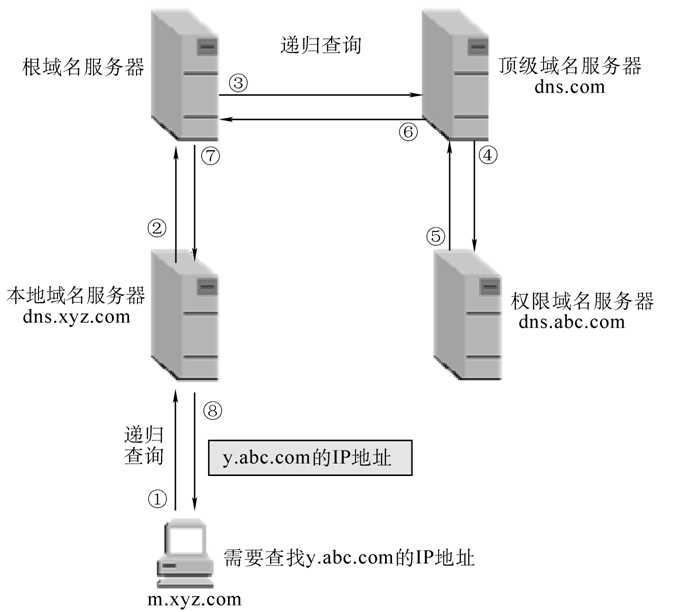
\includegraphics[width=6in]{png-jpeg-pics/8BC04566CF2B949C03E49D646B151CB9.png}
